En HiFi-forstærker kan være opbygget på forskellige måder, som blandt andet er afhængig af kravene til den. Når en HiFi-forstærker designes skal der stilles krav til funktionaliteten på brugerniveau såvel som det tekniske niveau, som brugeren ikke kommer i kontakt med. 
På brugerniveauet skal der foretages valg om hvilke indgangstyper HiFi-forstærkeren skal understøtte, udgangseffekten, kommunikation med brugeren, mulighed for justering af lydgengivelsen med mere. På det tekniske niveau skal der tages stilling til forvrængning, design af udgangstrin, type og styring af display med mere. 
For at anskueliggøre den grundlæggende opbygning af en HiFi-forstærker er figur \ref{fig:forstaerker_opbygning} opstillet.

\begin{figure}[h]
\centering
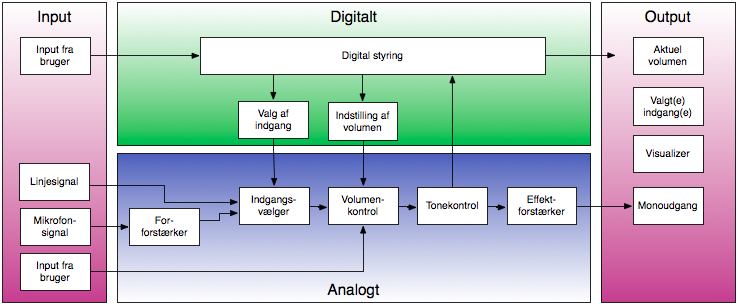
\includegraphics[scale=1]{indledende_analyse/generel_effektforstaerker/forstaerker_opbygning.png}
\caption{Opbygning af HiFi-forstærker}
\label{fig:forstaerker_opbygning}
\end{figure}

Kravene til dette projekts HiFi-forstærker vil i den resterende del af dette kapitel blive dokumenteret i form af en redegørelse for de valg der er blevet truffet. I kapitel \ref{kravspec} vil kravene være opstillet i en kravspecifikation.